\documentclass[journal,12pt,onecolumn]{IEEEtran}
\usepackage{cite}
\usepackage{amsmath,amssymb,amsfonts,amsthm}
\usepackage{algorithmic}
\usepackage{graphicx}
\usepackage{textcomp}
\usepackage{xcolor}
\usepackage{txfonts}
\usepackage{listings}
\usepackage{circuitikz}
\usepackage{enumitem}
\usepackage{mathtools}
\usepackage{gensymb}
\usepackage{comment}
\usepackage[breaklinks=true]{hyperref}
\usepackage{tkz-euclide} 
\usepackage{gvv}                                        
\usepackage[latin1]{inputenc}                                
\usepackage{color}                                            
\usepackage{array}                                            
\usepackage{longtable}                                       
\usepackage{calc}                                             
\usepackage{multirow}                                         
\usepackage{hhline}                                           
\usepackage{ifthen}                                           
\usepackage{lscape}
\usepackage{tabularx}
\usepackage{array}
\usepackage{float}
\usepackage{multicol}
\usepackage{caption}
\usetikzlibrary{patterns}

\newtheorem{theorem}{Theorem}[section]
\newtheorem{problem}{Problem}
\newtheorem{proposition}{Proposition}[section]
\newtheorem{lemma}{Lemma}[section]
\newtheorem{corollary}[theorem]{Corollary}
\newtheorem{example}{Example}[section]
\newtheorem{definition}[problem]{Definition}
\newcommand{\BEQA}{\begin{eqnarray}}
\newcommand{\EEQA}{\end{eqnarray}}
\newcommand{\define}{\stackrel{\triangle}{=}}
\theoremstyle{remark}
\newtheorem{rem}{Remark}

% Marks the beginning of the document
\begin{document}
\bibliographystyle{IEEEtran}
\vspace{3cm}

\title{Assignment 8}
\author{DESABOINA SRI SATHWIK-AI24BTECH11007}
\maketitle
% Removed \newpage to avoid a blank first page
\bigskip

\section*{GATE-2012:ME}
\label{}
\begin{enumerate}
    \item A large tank with a nozzle attached contains three immiscible, inviscid fluids as shown. Assuming that the changes in $h_1$, $h_2$ and $h_3$ are negligible, the instantaneous discharge velocity is
	    \vspace{1cm}
    \begin{center}
	    
\begin{circuitikz}
    % Define the nodes and draw the circuit
    \draw
    % MOSFET transistor with labels
    (0,0) node[nmos, anchor=S] (M) {}

    % Source resistor to ground
    (M.S) -- ++(0,-1) 
    to[R=500~$\Omega$] ++(0,-1) node[ground]{}

    % Gate resistor to ground
    (M.G) -- ++(-1,0) 
    to[R=2~M$\Omega$] ++(0,-2) node[ground]{}

    % Drain resistor to power supply
    (M.D) -- ++(0,1) 
    to[R=5~k$\Omega$] ++(0,1) 
    -- ++(0,0.5) node[vsource, rotate=0] {25 V};

    % Draw a large circle around the NMOS transistor
    \draw[thick] (M) circle (1cm); % Adjust the radius as needed
    
    % Draw a small circle at the other end of the 5 kΩ resistor (connected to the voltage source)
    \draw[thick] ++(0, 3.7) circle (0.15cm); % Small circle at the top end of the 5 kΩ resistor

\end{circuitikz}


    \end{center}
	    \hfill{(ME:2012)}
		\begin{multicols}{2}
    \begin{enumerate}
        \item $ \sqrt{2g \left( \frac{\rho_1 h_1 + \rho_2 h_2 + \rho_3 h_3}{\rho_3 h_3} \right)} $
        \item $\sqrt{2g(h_1 + h_2 + h_3)}$
	\item $\sqrt{2g (\frac{\rho_1 h_1 + \rho_2 h_2 + \rho_3 h_3}{\rho_1 + \rho_2 + \rho_3})}$
	\item $\sqrt{2g (\frac{\rho_1 h_2 h_3 + \rho_2 h_1 h_3 + \rho_3 h_1 h_2}{\rho_1 h_1 + \rho_2 h_2 + \rho_3 h_3})}$
    \end{enumerate}
		\end{multicols}

    \item Water $(C_p = 4.18 \, kJ/kg.K)$ at $80^\circ C$ enters a counterflow heat exchanger with a mass flow rate of $0.5 \, kg/s$. Air $(C_p = 1 \, kJ/kg.K)$ enters at $30^\circ C$ with a mass flow rate of $2.09 \, kg/s$. If the effectiveness of the heat exchanger is 0.8, the LMTD (in $^\circ C$) is

	     \hfill{(ME:2012)}
		\begin{multicols}{4}
    \begin{enumerate}
        \item $40$
        \item $20$
        \item $10$
        \item $5$
    \end{enumerate}
\end{multicols}

    \item A solid steel cube constrained on all six faces is heated so that the temperature rises uniformly by $\Delta T$. If the thermal coefficient of the material is $\alpha$, Young's modulus is $E$ and the Poisson's ratio is $\nu$, the thermal stress developed in the cube due to heating is

	     \hfill{(ME:2012)}
		\begin{multicols}{4}
    \begin{enumerate}
	    \item $-\frac{\alpha E \Delta T}{(1 - 2\nu)}$
	    \item $-\frac{2 \alpha E \Delta T}{(1 - 2\nu)}$
	    \item $-\frac{3 \alpha E \Delta T}{(1 - 2\nu)}$
        \item $-\frac{\alpha E \Delta T}{3(1 - 2\nu)}$
    \end{enumerate}
		\end{multicols}

    \item 
	    A solid circular shaft needs to be designed to transmit a torque of $50 \, N.m$. If the allowable shear stress of the material is $140 \, MPa$, assuming a factor of safety of $2$, the minimum allowable design diameter in $mm$ is

		 \hfill{(ME:2012)}
		\begin{multicols}{4}
    \begin{enumerate}
        \item $8$
        \item $16$
        \item $24$
        \item $32$
    \end{enumerate}
		\end{multicols}

    \item 
	    A force of $400 \, N$ is applied to the brake drum of $0.5 \, m$ diameter in a band-brake system as shown in the figure, where the wrapping angle is $180^\circ$. If the coefficient of friction between the drum and the band is 0.25, the braking torque applied, in $N.m$ is
		\vspace{1cm}
		\begin{center}
			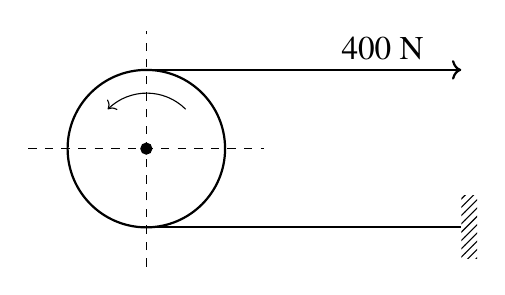
\begin{tikzpicture}
    % Draw the circle
    \draw[thick] (0,0) circle(1);
    
    % Draw the center point and dashed lines
    \draw[dashed] (-1.5,0) -- (1.5,0);
    \draw[dashed] (0,-1.5) -- (0,1.5);
    \filldraw (0,0) circle (2pt);

    % Draw the rotational arrow
    \draw[->] (0.5,0.5) arc[start angle=45, end angle=135, radius=0.7];

    % Draw the 400 N force arrow
    \draw[thick, ->] (0,1) -- (4,1) node[near end, above] {\large $400\ \text{N}$};

    % Draw the fixed support on the right
    \draw[thick] (0, -1) -- (4, -1);
    \fill[pattern=north east lines] (4.2, -1.4) rectangle (4, -0.6);
\end{tikzpicture}

		\end{center}

		 \hfill{(ME:2012)}
\begin{multicols}{4}
    \begin{enumerate}
        \item $100.6$
        \item $54.4$
        \item $22.1$
        \item $15.7$
    \end{enumerate}
\end{multicols}

    \item A box contains $4$ red balls and $6$ black balls. Three balls are selected randomly from the box one after another, without replacement. The probability that the selected set contains one red ball and two black balls is

	     \hfill{(ME:2012)}
\begin{multicols}{4}
    \begin{enumerate}
        \item $\frac{1}{20}$
        \item $\frac{1}{12}$
        \item $\frac{3}{10}$
        \item $\frac{1}{2}$
    \end{enumerate}
\end{multicols}

    \item 
	    Consider the differential equation
   $ x^2 \frac{d^2y}{dx^2} + 4x \frac{dy}{dx} - 4y = 0$
    with the boundary conditions of $y(0) = 0$ and $y(1) = 1$. The complete solution of the differential equation is

     \hfill{(ME:2012)}
\begin{multicols}{4}
    \begin{enumerate}
        \item $x^2$
	\item $\sin (\frac{\pi x}{2})$
	\item $e^x \sin (\frac{\pi x}{2})$
	\item $e^{-x} \sin (\frac{\pi x}{2})$
    \end{enumerate}
\end{multicols}

    \item
$x + 2y + z = 4 \\
2x + y + 2z = 5 \\
x - y + z = 1$\\
    The system of algebraic equations given above has

     \hfill{(ME:2012)}
    \begin{enumerate}
        \item a unique solution of $x = 1, y = 1$ and $z = 1$.
        \item only the two solutions of $(x = 1, y = 1, z = 1)$ and $(x = 2, y = 1, z = 0)$.
        \item infinite number of solutions.
        \item no feasible solution.
    \end{enumerate}
\vspace{0.5cm}
     \textbf{Common data for questions \ref{a} and \ref{b}} \\ 
    Two steel truss members, $AC$ and $BC$, each having cross-sectional area of $100 \, {mm}^2$, are subjected to a horizontal force $F$ as shown in figure. All the joints are hinged.
    \begin{center}
	    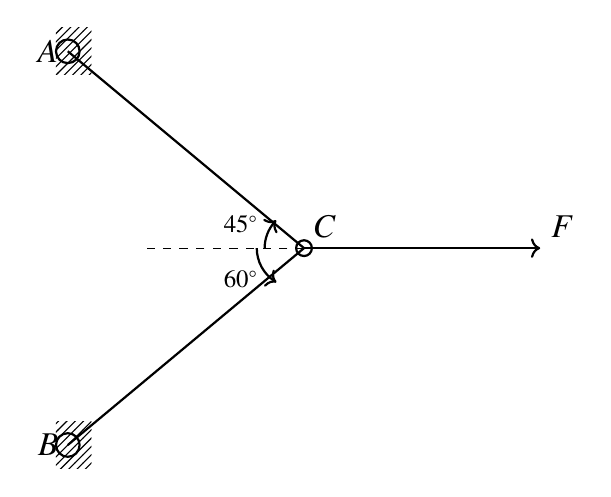
\begin{tikzpicture}
    % Define points with A and B further left and spaced vertically
    \coordinate (A) at (-3,2.5);
    \coordinate (B) at (-3,-2.5);
    \coordinate (C) at (0,0);
    \coordinate (F) at (3,0);

    % Draw fixed supports at A and B
    \fill[pattern=north east lines] (-3.15,2.8) rectangle (-2.7,2.2);
    \fill[pattern=north east lines] (-3.15,-2.2) rectangle (-2.7,-2.8);
    
    % Draw circles at supports
    \draw[thick] (A) circle(0.15);
    \draw[thick] (B) circle(0.15);
    \draw[thick] (C) circle(0.1);

    % Draw the rods AC and BC
    \draw[thick] (A) -- (C);
    \draw[thick] (B) -- (C);

    % Draw force arrow at C and label at the end
    \draw[thick, ->] (C) -- (F) node[above right] {\large $F$};

    % Draw a dashed line from C to the left
    \draw[dashed] (C) -- ++(-2,0);

    % Draw angle arcs and labels in correct positions
    \draw[thick, ->] (-0.5,0) arc[start angle=180, end angle=135, radius=0.5];
    \node at (-0.8,0.3) {\small $45^\circ$};
    
    \draw[thick, ->] (-0.6,0) arc[start angle=180, end angle=240, radius=0.5];
    \node at (-0.8,-0.4) {\small $60^\circ$};

    % Label points A, B, and C
    \node[left] at (A) {\large $A$};
    \node[left] at (B) {\large $B$};
    \node[above right] at (C) {\large $C$};

\end{tikzpicture}

    \end{center}

     \hfill{(ME:2012)}

        \item
		If $F = 1 \, kN$, the magnitude of the vertical reaction force developed at the point $B$ in $kN$ is
		\label{a}
		\begin{multicols}{4}
        \begin{enumerate}
            \item $0.63$
            \item $0.32$
            \item $1.26$
            \item $1.46$
        \end{enumerate}
		\end{multicols}
        \item
		The maximum force $F$ in kN that can be applied at $C$ such that the axial stress in any of the truss members DOES NOT exceed $100 \, MPa$ is
		\label{b}
		\begin{multicols}{4}
        \begin{enumerate}	
            \item $8.17$
            \item $11.15$
            \item $14.14$
            \item $22.30$
        \end{enumerate}
	\end{multicols}
\vspace{0.5cm}
     \textbf{Common data for questions \ref{c} and \ref{d}} \\ 
    A refrigerator operates between $120 \, kPa$ and $800 \, kPa$ in an ideal vapor compression cycle with $R-134a$ as the refrigerant. The refrigerant enters the compressor as saturated vapor and leaves the condenser as saturated liquid. The mass flow rate of the refrigerant is $0.2 \, kg/s$. Properties for $R-134a$ are as follows:
    \vspace{0.01cm}
    \begin{table}[h!]
\centering
\caption*{Saturated R-134a Properties}
\begin{tabular}{|c|c|c|c|c|c|}
\hline
$P$ (kPa) & $T$ ($^\circ$C) & $h_f$ (kJ/kg) & $h_g$ (kJ/kg) & $s_f$ (kJ/kg$\cdot$K) & $s_g$ (kJ/kg$\cdot$K) \\
\hline
120 & -22.32 & 22.5 & 237 & 0.093 & 0.95 \\
800 & 31.31  & 95.5 & 267.3 & 0.354 & 0.918 \\
\hline
\end{tabular}
\end{table}

    \vspace{0.1cm}
    \begin{table}[h!]
\centering
\caption*{Superheated R-134a Properties}
\begin{tabular}{|c|c|c|c|}
\hline
$P$ (kPa) & $T$ ($^\circ$C) & $h$ (kJ/kg) & $s$ (kJ/kg$\cdot$K) \\
\hline
800 & 40 & 276.45 & 0.95 \\
\hline
\end{tabular}
\end{table}


     \hfill{(ME:2012)}

        \item
		The rate at which heat is extracted, in $kJ/s$ from the refrigerated space is
		\label{c}
		\begin{multicols}{4}
        \begin{enumerate}
            \item $28.3$
            \item $42.9$
            \item $34.4$
            \item $14.6$
        \end{enumerate}
		\end{multicols}

        \item
		The power required for the compressor in $kW$ is
		\label{d}
		\begin{multicols}{4}
        \begin{enumerate}
            \item $5.94$
            \item $1.83$
            \item $7.9$
            \item $39.5$
        \end{enumerate}
		\end{multicols}
\vspace{0.5cm}
    \textbf{Linked Answer Questions:}\\
    Air enters an adiabatic nozzle at $300 \, kPa, 500 \, K$ with a velocity of $10 \, m/s$. It leaves the nozzle at $100 \, kPa$ with a velocity of $180 \, m/s$. The inlet area is $80 \, {cm}^2$. The specific heat of air $C_p$ is $1008 \, J/kg.K$.

     \hfill{(ME:2012)}

        \item
		The exit temperature of the air is
		\begin{multicols}{4}
        \begin{enumerate}
            \item $516 \, K$
            \item $532 \, K$
            \item $484 \, K$
            \item $468 \, K$
        \end{enumerate}
		\end{multicols}
\end{enumerate}
\end{document}

